\chapter{\positron\electron pair background as the largest background contribution}
\label{PairBkg}

\begin{chapterabstract}
 At the International Linear Collider, the collision of the two lepton beams goes hand in hand with the production of background particles.
 Unlike at hadron colliders, the main background contribution does not arise from QCD processes and underlying events, but rather from the interaction of the colliding beam's electromagnetic fields.
 The created secondary \positron\electron pairs form a significant background, the so-called pair background, for the inner detectors, and therefore need to be studied in great detail.
 This chapter discusses the effect of the ILC beam parameters on the pair background, and the impact of the \positron\electron pairs on the \sid detector.
\end{chapterabstract}

As discussed in Section~\ref{BeamBeam}, the pair background is a high cross section process from beam-beam interactions and the main source of background at the ILC.
The secondary electrons and positrons show a characteristic density distribution, which reach to the inner layers of the \sid vertex and tracking detectors.
The impact on the \sid detector is studied with respect to the timing, the hit distribution, and the arising detector occupancy.
These impacts are, however, affected by the change in the ILC beam parameters for the ILC250 stage, which is another study done for this thesis and is explained throughout the following sections.
The results of these studies contributed towards design choices of the accelerator and the \sid detector.

\section{The background generator GuineaPig}
\label{PairBkg:GuineaPig}
For studying the effects of the pair background, \positron\electron pairs from beam-beam interactions were generated with the Monte Carlo (MC) background event generator \guineapig~\cite{Schulte:1997nga} version 1.4.4. 
When providing the accelerator beam parameters, the pair background events of one bunch crossing are simulated and stored in an ASCII output file named ``pairs.dat''.
The parameters used for generating the pair background for this thesis are given in Appendix~\ref{Appendix:Pairs:GuineaPig}. 
\\Since the ASCII files cannot directly serve as input to a full \geant~\cite{geant_ref,geant_ref2} detector simulation, a conversion tool was written in context of this thesis, and instructions on its usage are available in~\cite{Confluence}. 
The tool converts the ASCII output to one of the following common file formats: stdhep or slcio~\cite{LCIO}.
These file formats are directly applicable with the \geant based simulation tool \slic~\cite{Graf:2006ei}, which simulates interactions of the input particles with matter.
The geometry of the simulated world is described in a lcdd file in a human-readable format.
The flexible geometry description allows the simulation of particle interactions with individual detector geometries.
To this end, the geometry description file ``sidloi3'' of the \sid detector, which was used for the simulation studies in this and in the following chapters, is based on the detector design described in Section~\ref{ILC:SiD} and in~\cite[p. 69 ff]{TDR4}.

\section{Pair background envelopes}
\label{PairBkg:helix}
Analyzing the generated pair background events, it becomes apparent that the \positron\electron pairs have a low transverse momentum.
Figure~\ref{fig:PairBkg:Momentum} shows the distribution of their longitudinal and transverse momentum for the two ILC stages at \SI{250}{\GeV} and \SI{500}{\GeV} center-of-mass energy.
The longitunal momentum of the \positron\electron pairs reaches roughly \SI{80}{\percent} of the beam energy, whilst the transverse momentum extends to only \SI{0.8}{\GeV} for the ILC250, and \SI{1.6}{\GeV} for the ILC500.
 \begin{figure}[h]
 \centering
  \begin{subfigure}[b]{0.49\textwidth}
   \centering
    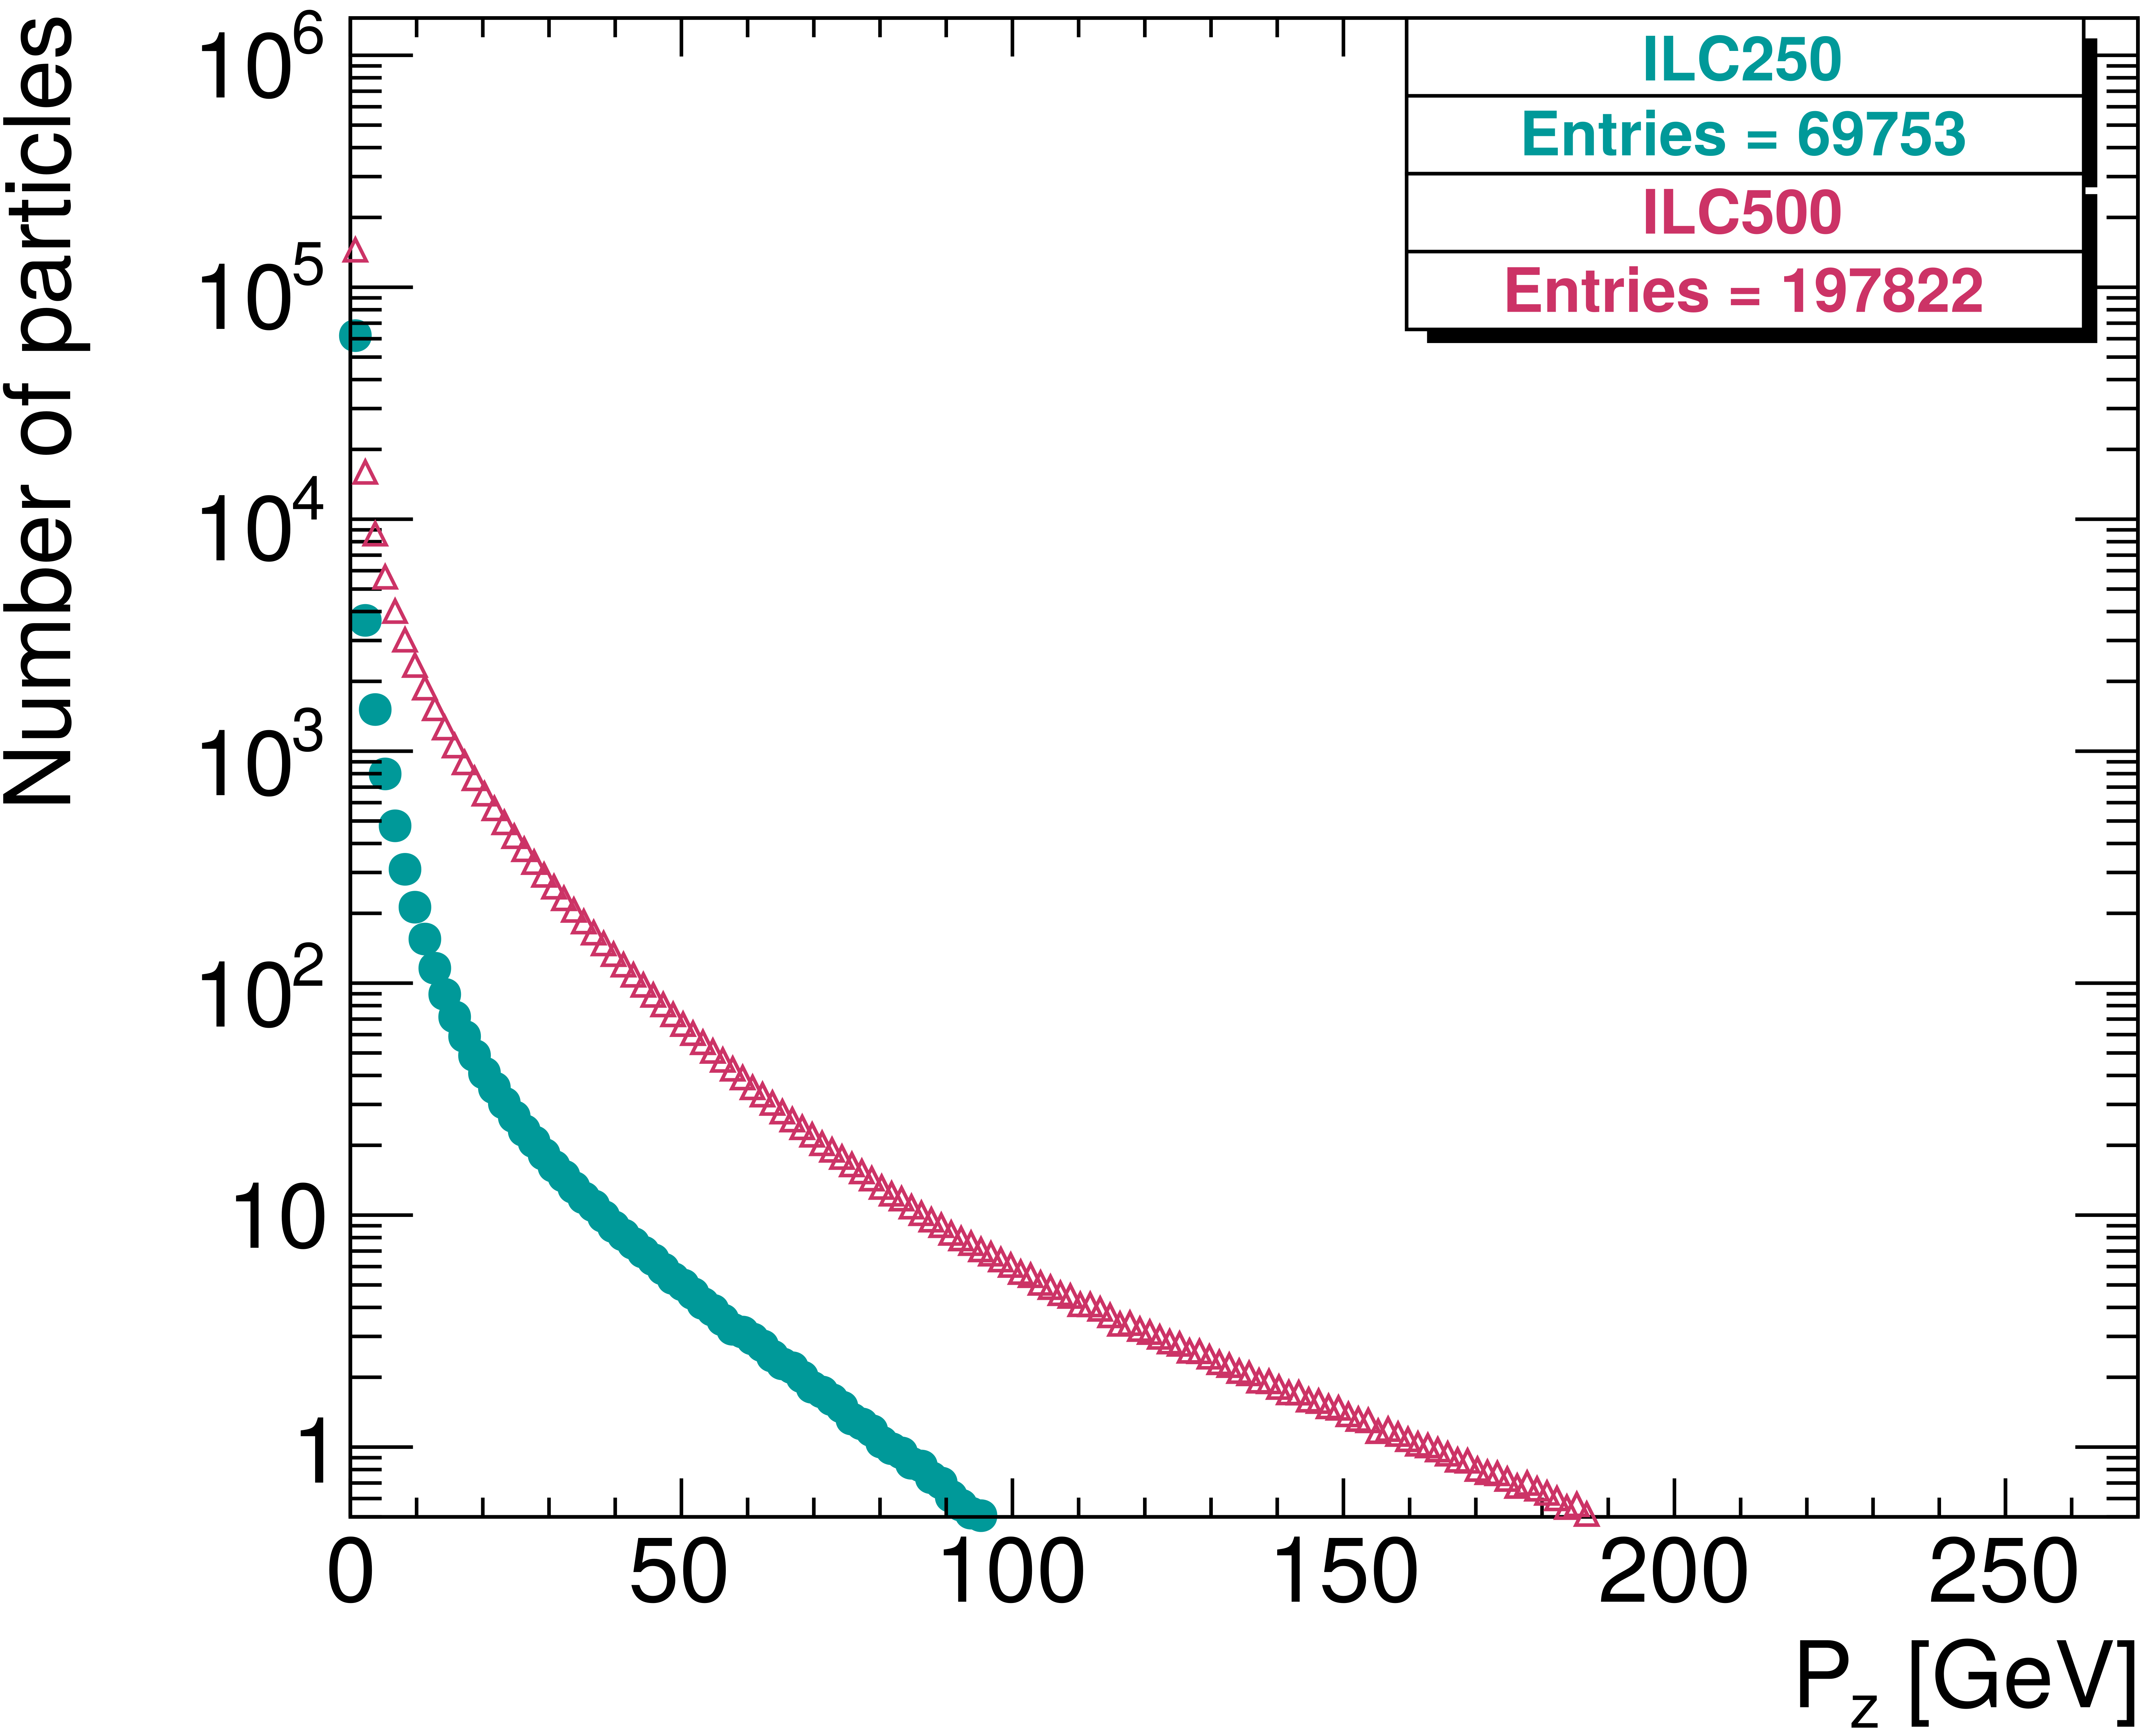
\includegraphics[width=0.95\textwidth]{Figures/Pairs/250_500_pairs_comparison_Pz.png}
   \caption{Longitudinal momentum}
   \end{subfigure}
   \hfill
    \begin{subfigure}[b]{0.49\textwidth}
   \centering
    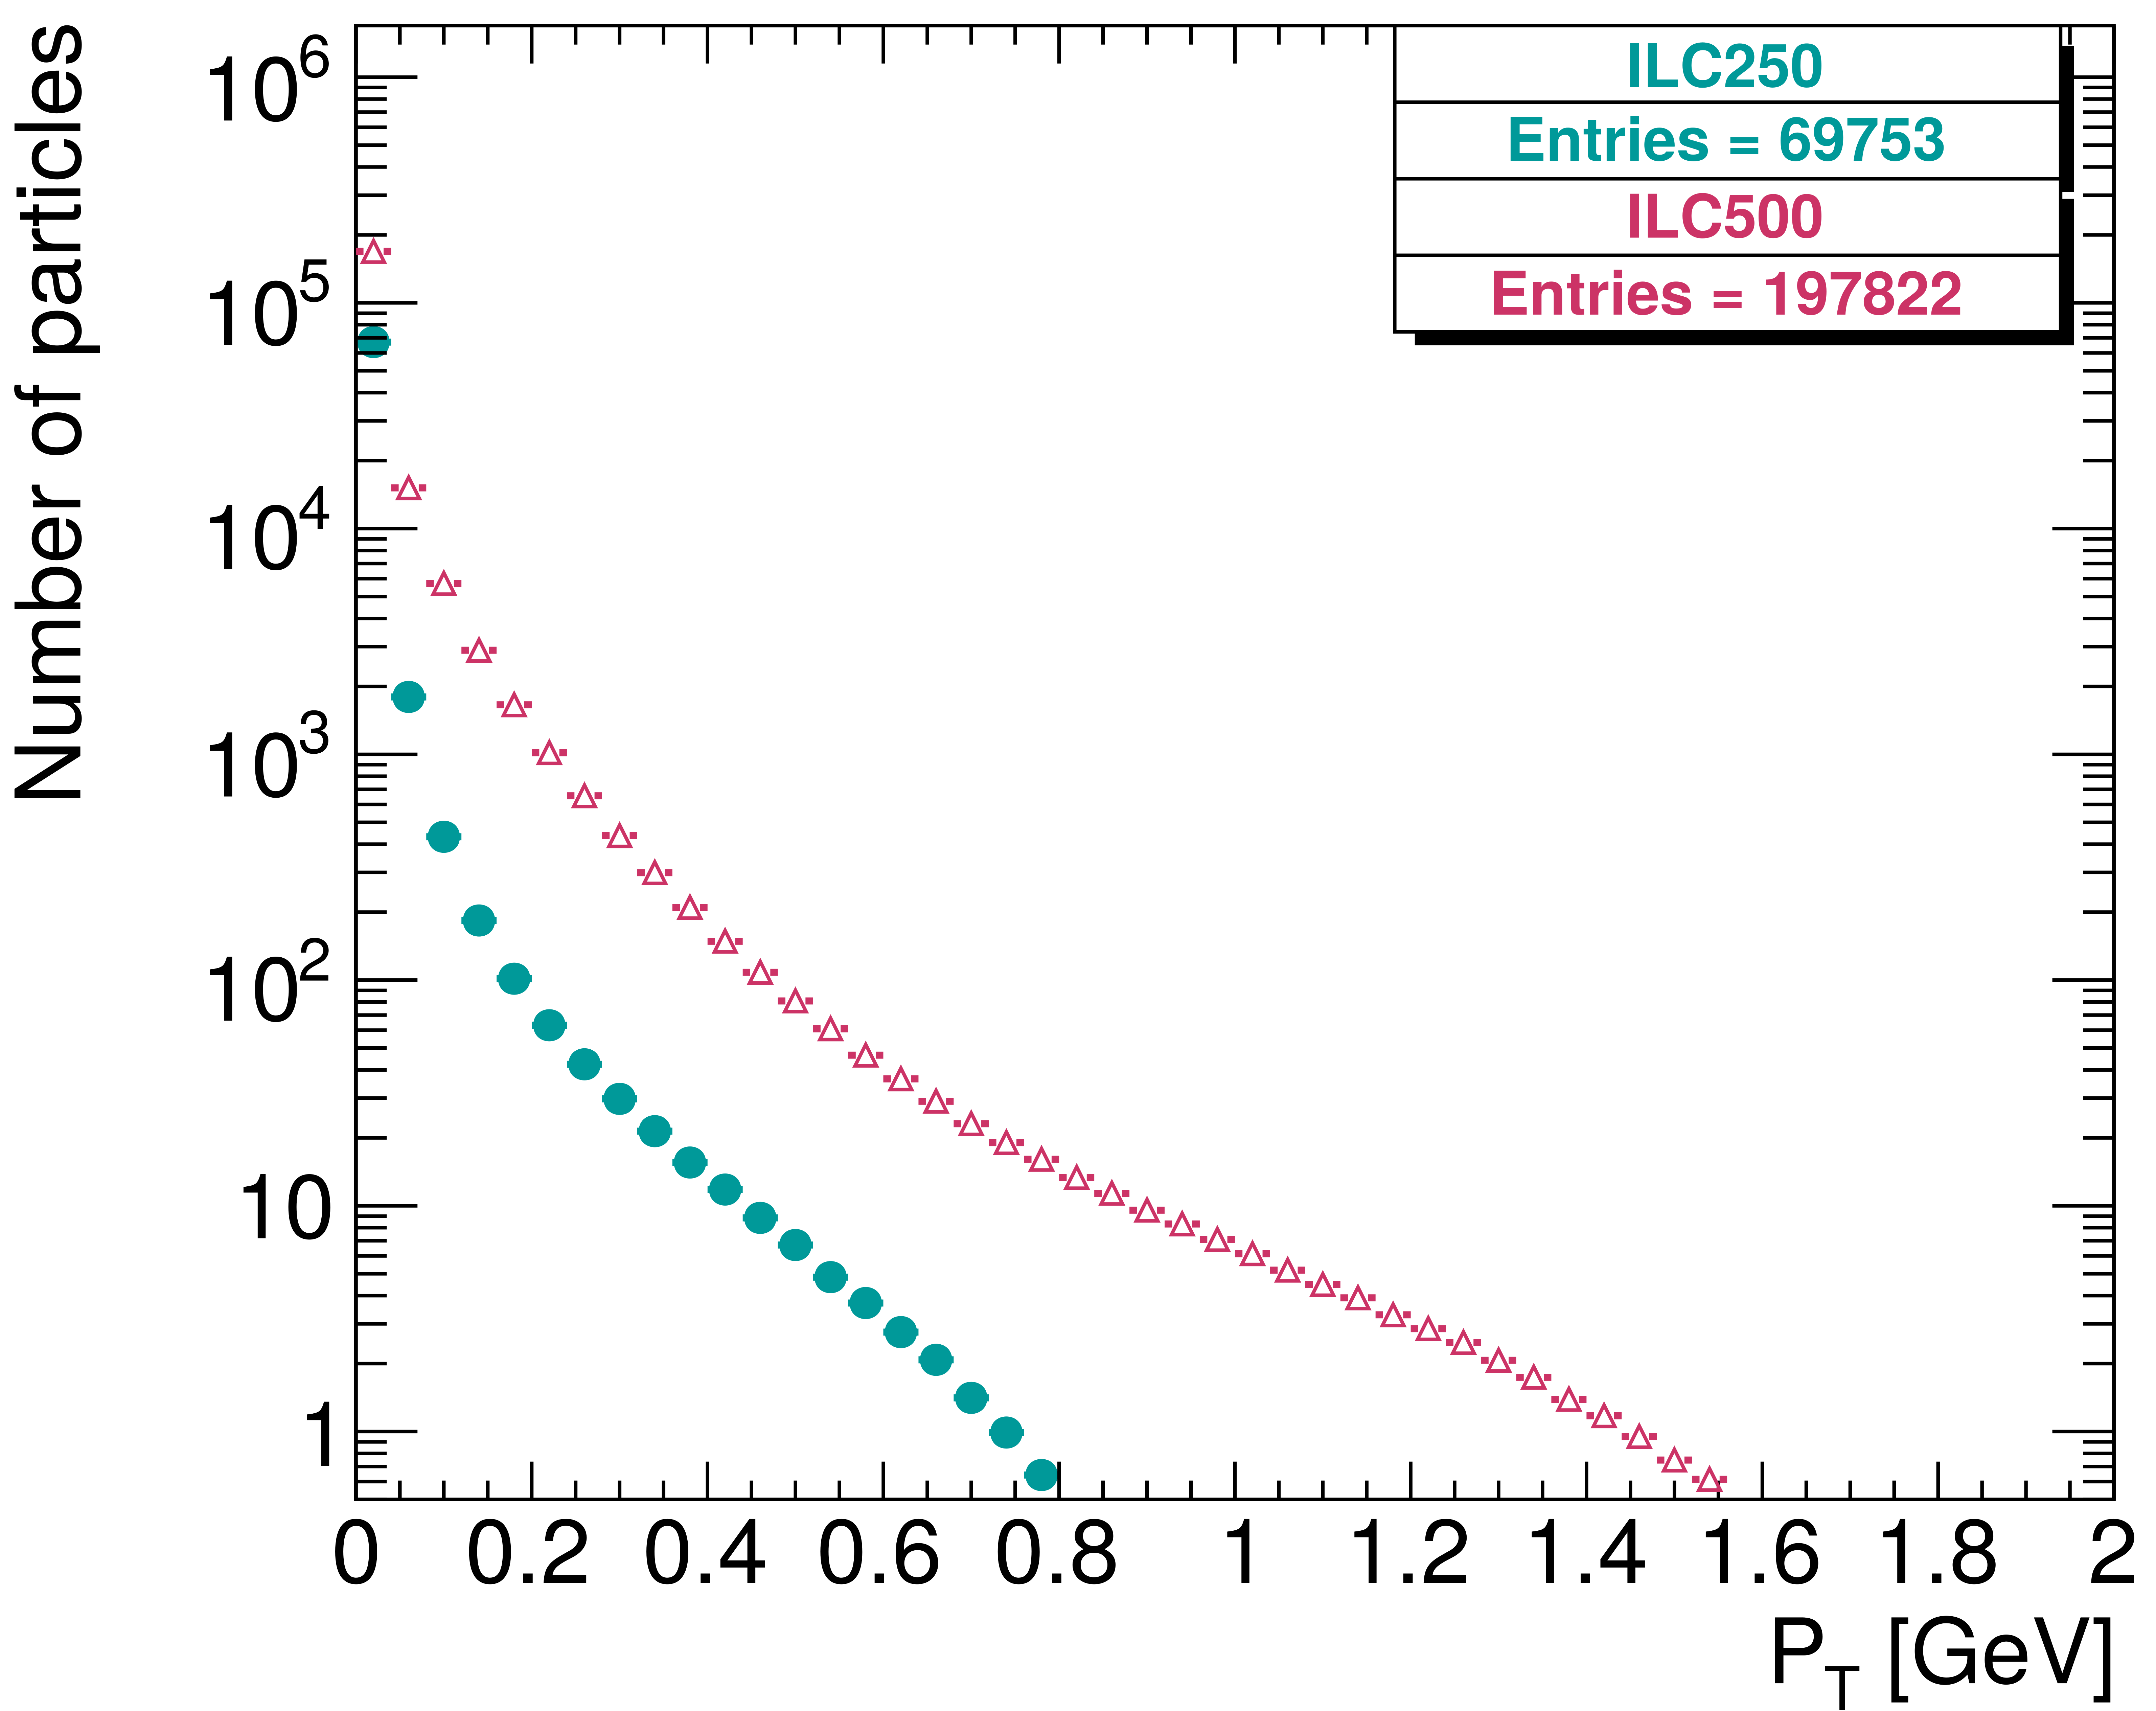
\includegraphics[width=0.96\textwidth]{Figures/Pairs/250_500_pairs_comparison_PT.png}
   \caption{Transverse momentum}
   \end{subfigure}
   \caption[Pair background momentum distributions]{Comparison of the pair background momentum distributions for the ILC at \SI{250}{\GeV} and \SI{250}{\GeV} center-of-mass energy, with the longitudinal momentum shown in Figure (a) and the transverse momentum in Figure (b).}
   \label{fig:PairBkg:Momentum}
 \end{figure}
\\Due to their low transverse momentum, the pairs are deflected on helical tracks in the magnetic field of the detector solenoid magnet.
An algorithm was written that calculates the helix tracks of the pair particles using their four-vectors.
The track positions are computed from the radius of the helix, its center position and its pitch. The following assumptions were made for the algorithm:
The magnetic field in the proximity of the IP is homogeneous, with a field strength of \SI{5}{\tesla} for the SiD solenoid.
The particle momenta do not change in the region of interest for this analysis, because of which the helix radius is constant.
Any particle interaction with other particles or with matter is not taken into account.
\\Figure~\ref{fig:helix_circle} shows schematically the projection of a helix onto the xy-plane.
Depending on the particle's charge the orientation of the helix is determined.
\begin{figure}
    \centering
    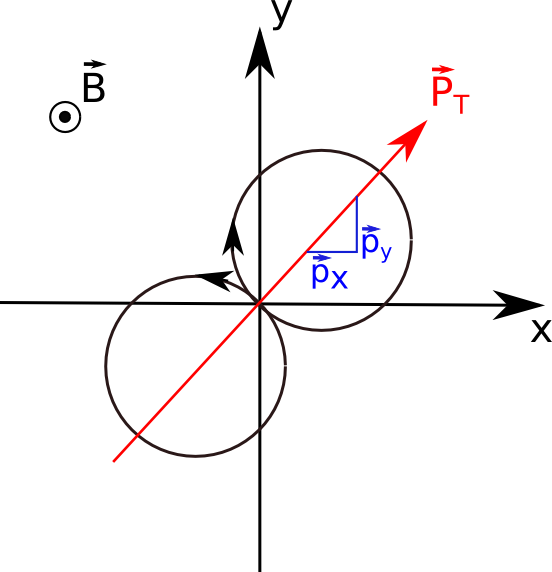
\includegraphics[width=0.3\textwidth]{Figures/Pairs/Helix_explanation.png}
    \caption[Schematic projection of the helix on the xy-plane]{
    This schematic shows the projection of a helix track onto the xy-plane, with the vector of the transverse momentum (P\textsubscript{T}) and the the x- and y-momenta (p\textsubscript{x} and p\textsubscript{y}).
    Depending on the particle's charge, the direction of the rotation is either clockwise or anticlockwise.
    The center, the radius, and the orientation of the projected circle is dependent on the transverse momentum of the particle.
    }
    \label{fig:helix_circle}
\end{figure}
The pair density is then plotted using the helix track algorithm to calculate the position in x and y for a given position in z.
For the ILC stage at \SI{500}{\GeV}, the pair background was generated with \guineapig, and its density plotted in Figure~\ref{fig:PairBkg:Density} (a).
The density distribution of all the tracks shows a characteristic bell shape, with the highest density along the z axis.
Since the bell shaped envelope is fully symmetrical in positive and negative z-direction as well as in the xz and yz-plane, the chosen view of the pair background envelopes will in the following always be of the xz-plane in positive z-direction.
 \begin{figure}[!h]
 \centering
  \begin{subfigure}[b]{0.49\textwidth}
   \centering
    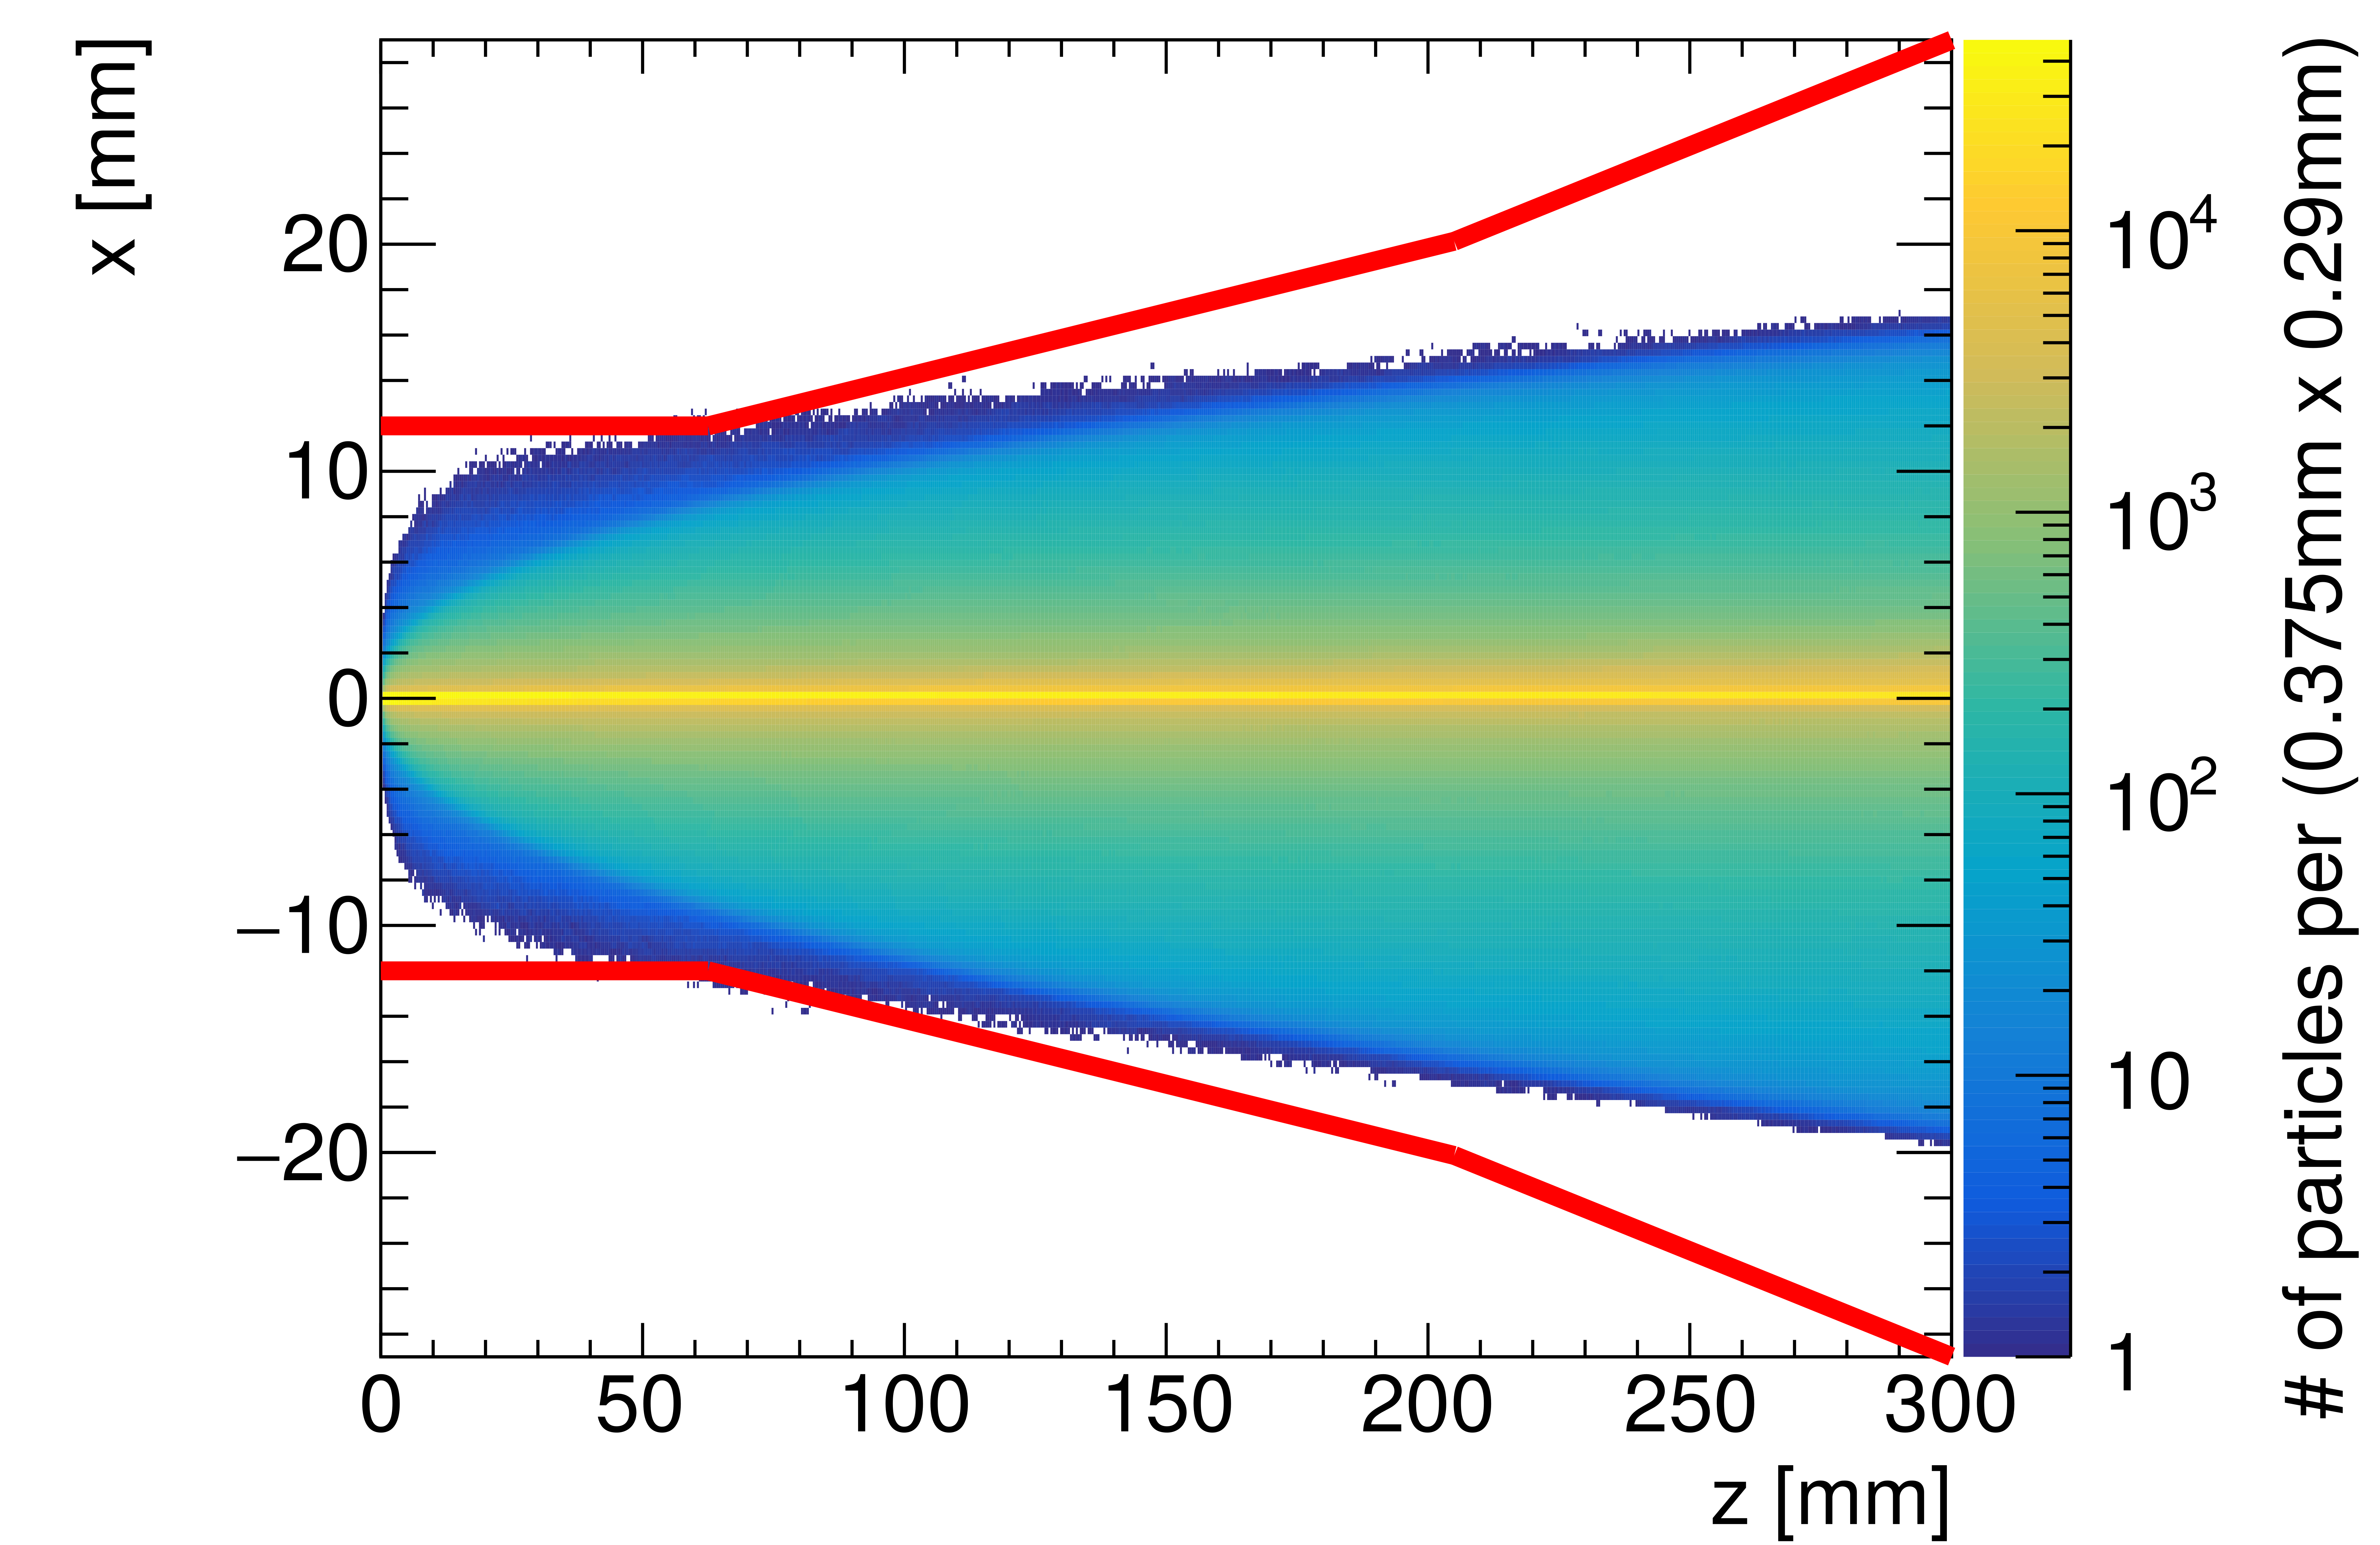
\includegraphics[width=\textwidth]{Figures/Pairs/Helix_tracks_xz_80bunches_500GeV_5T.png}
   \caption{Pair backgound density for the ILC500}
   \end{subfigure}
   \hfill
    \begin{subfigure}[b]{0.49\textwidth}
   \centering
    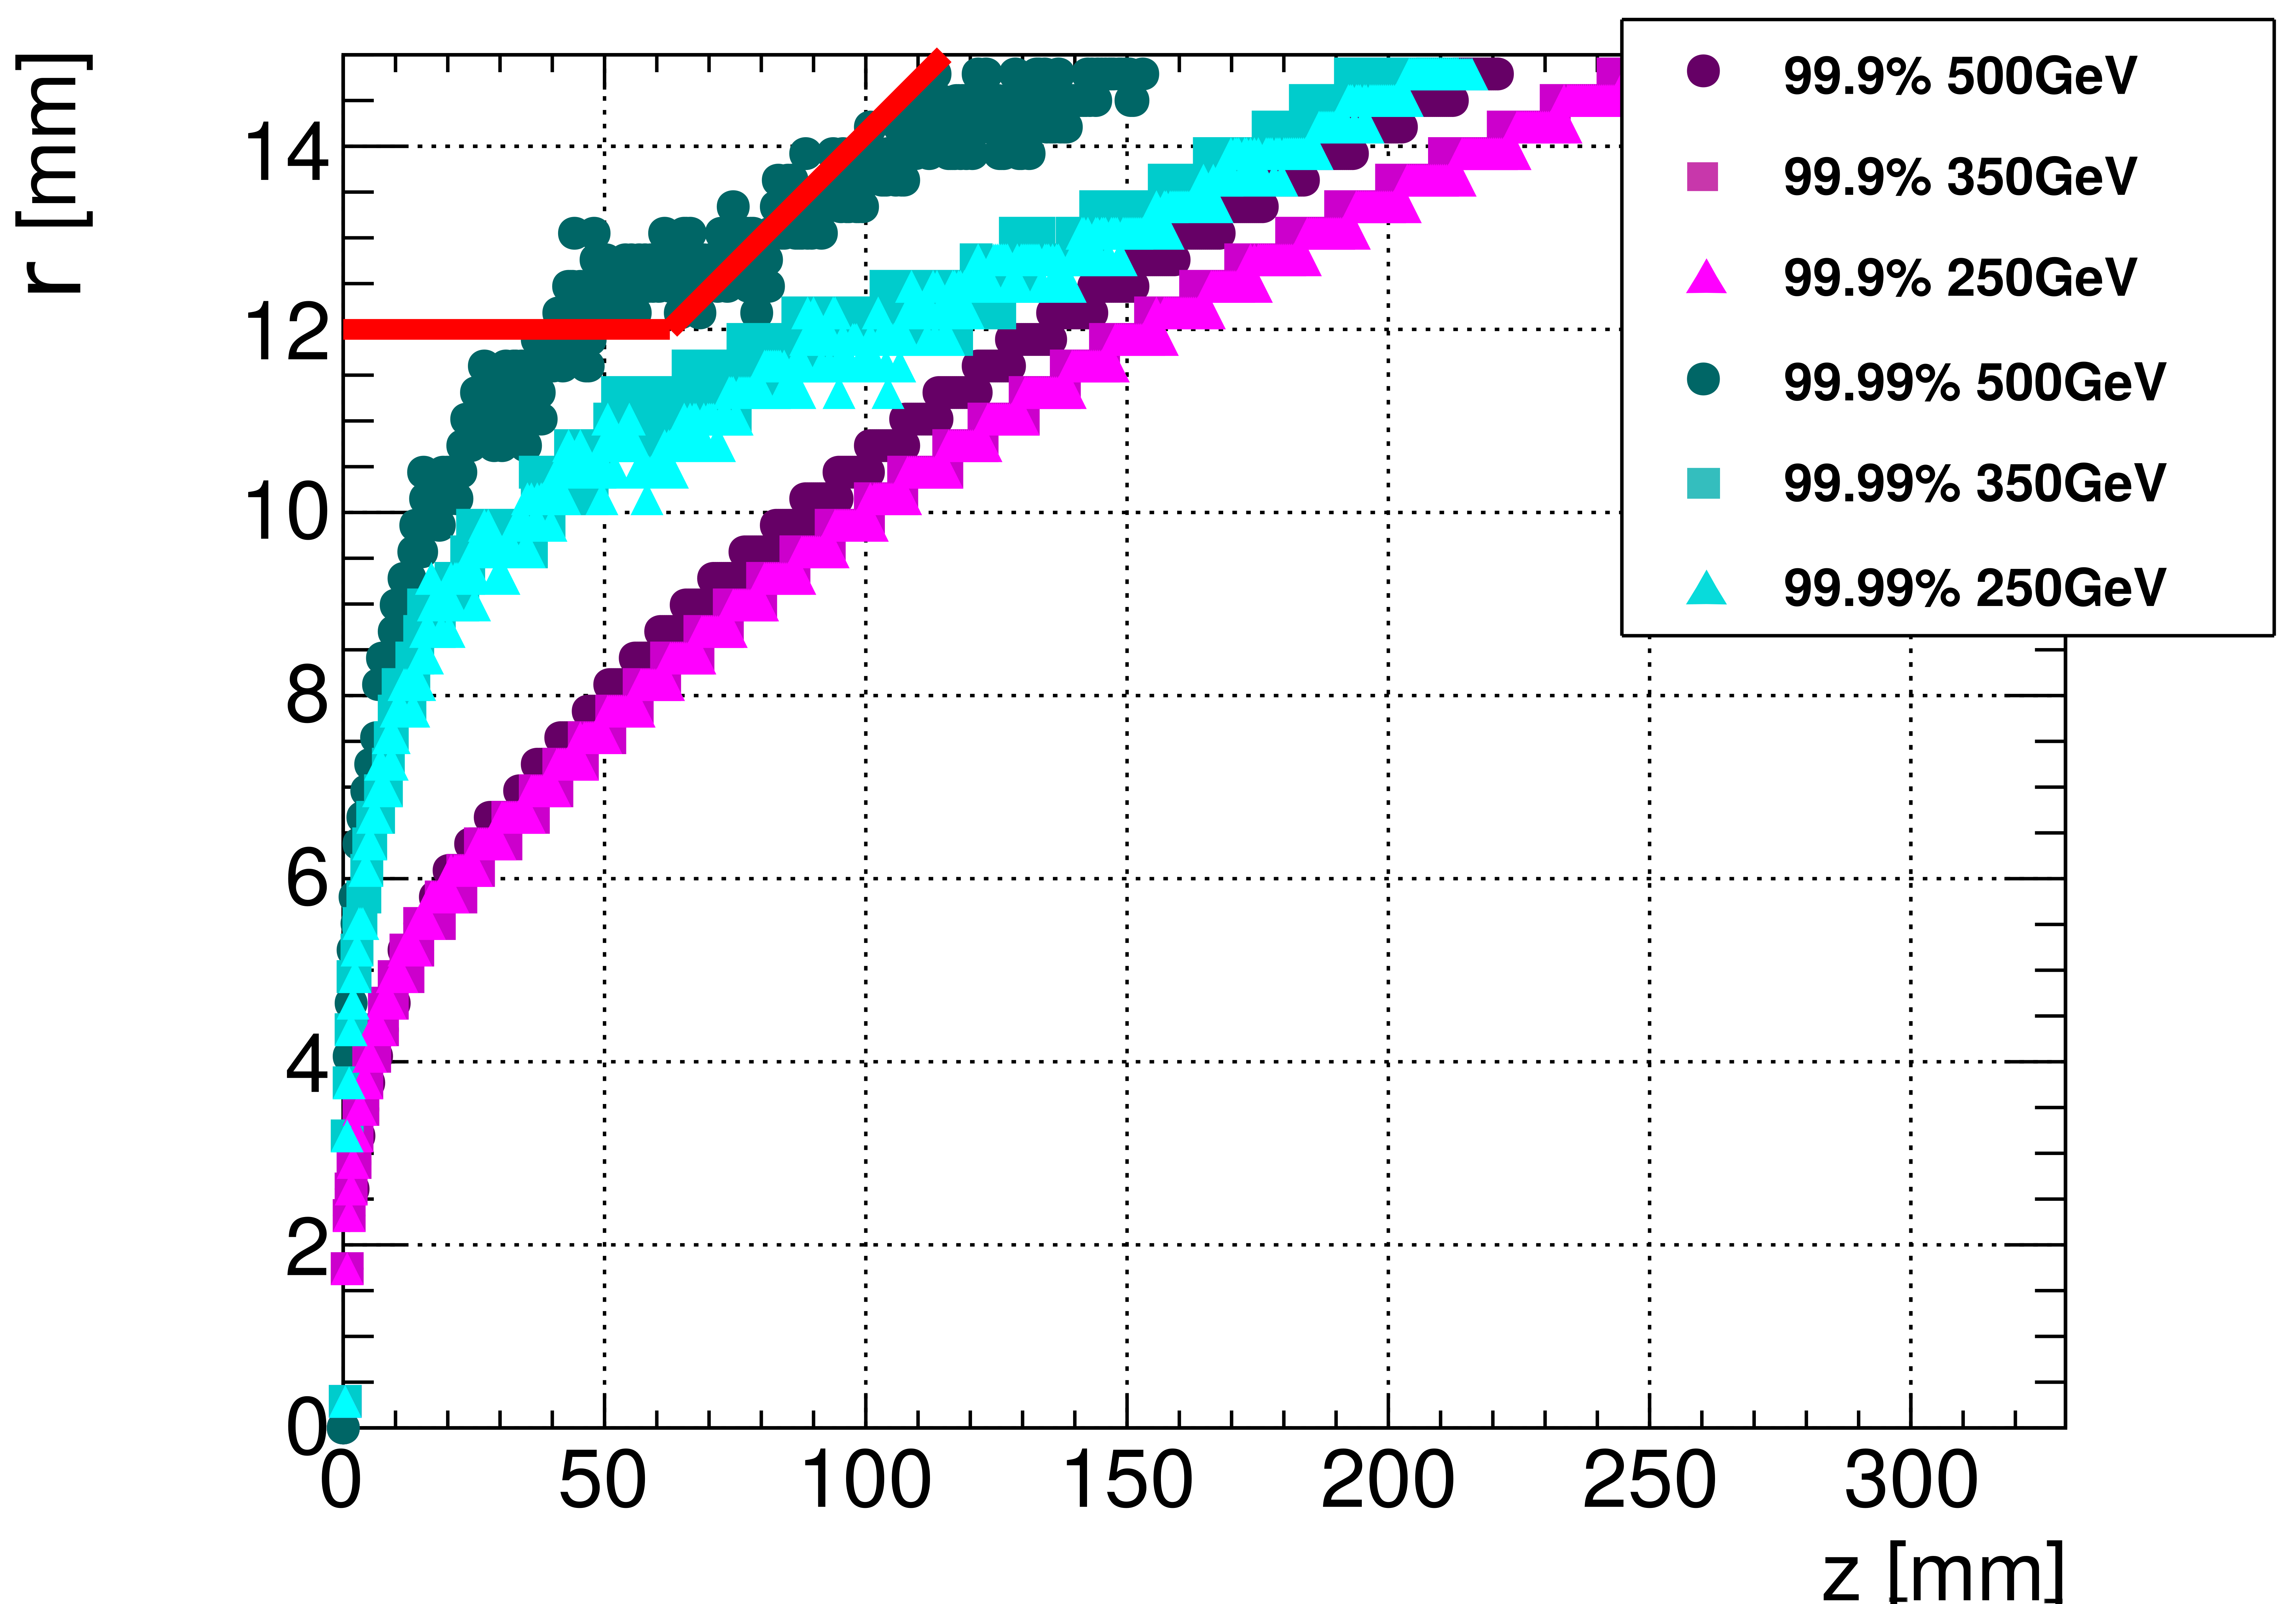
\includegraphics[width=\textwidth]{Figures/Pairs/HelixEnvelopes_COMPARISON_xz_500_350_250_comparison_EDITED_2.png}
   \caption{yz-plane}
   \end{subfigure}
   \caption[Pair background density]{The figures display the pair background density in the xz-plane for one ILC bunch crossing.
   Figure (a) shows the complete track density distribution of the pairs at the ILC stage at a center-of-mass energy of \SI[detect-all]{500}{\GeV}.
   The color scale shows the number of tracks per unit area.
   The red solid lines represent the outline of the beam pipe
   \\In Figure (b), the density envelopes of three ILC stages are compared: at 250, 350, and \SI[detect-all]{500}{\GeV}.
   For that purpose, not the complete density distribitution is plotted, but rather the envelope outlines containing either \SI[detect-all]{99.9}{\percent} or \SI[detect-all]{99.99}{\percent} of all tracks.
   }
   \label{fig:PairBkg:Density}
 \end{figure}
\\In order to compare the envelope shapes for different ILC beam parameters, Figure~\ref{fig:PairBkg:Density} (b) only shows the envelope outlines containing a certain fraction of all tracks.
In this way, it becomes apparent that for higher center-of-mass energies the width of the envelope increases due to the higher transversal momenta of the pairs.
At \SI{500}{\GeV}, the envelope containing \SI{99.99}{\percent} of all pair helix tracks crosses the beam pipe, extending towards the innermost layer of the SiD vertex detector, which has a radius of \SI{14}{\milli\meter}.
For lower center-of-mass energies, the envelopes stay within the beam pipe radius.
The pair background simulation files for this comparison plot were generated with \guineapig as well, using the beam parameters of the three different baseline ILC stages~\cite[p. 11]{TDR1}.
 
As explained in Section~\ref{ILC:layout:staging}, the first ILC stage will be at \SI{250}{\GeV} instead of the originally anticipated \SI{500}{\GeV}.
Due to this decision in 2017, efforts have been made to study a possible change in the baseline beam parameters for this stage in order to increase the luminosity from \num{8.2} to \SI{16.2e34}{\per\centi\meter\squared\per\second}~\cite{LCWS17_paper}. 
To this end, three alternative beam parameter sets have been suggested, which vary from the original baseline parameters in the emittance and the beta function values.
The values which differ are listed in Table~\ref{tab:ILC250_sets}.
For all alternative sets, the horizontal emittance $\epsilon_x$ is reduced. 
Additionally, the horizontal and vertical beta functions at the IP, $\beta^*_x$ and $\beta^*_y$, are changed for sets (B) and (C).
Since both, the emittance and the beta function, are dependencies of the beam size, they enter indirectly the Equation~\ref{eq:luminosity} for the beam luminosity.
\\On the other hand however, a reduced horizontal emittance implies also an increase in the beam-beam interactions and in the pair background level.
For the process of deciding the new official beam parameter set, a study of the impact of this increased pair background on the \sid vertex detector performance was therefore a crucial step.
In the following, the simulation studies of the pair background for the four parameter schemes listed in Table~\ref{tab:ILC250_sets} are presented.
\begin{table}[h]
\caption[New ILC250 beam parameters]{Changes between the baseline and alternative beam parameter sets for the ILC stage at \SI[detect-all]{250}{\GeV}~\cite{LCWS17_paper}.
The highlighted parameter set (A) was chosen to be the new official scheme for the ILC250.}
\label{tab:ILC250_sets}
\centering
\begin{tabularx}{0.48\textwidth}{c|ccc}
\hline\hline
\textbf{ILC250 sets} & $\epsilon_x$ (\si{\micro\meter}) & $\beta^*_x$ (\si{\milli\meter}) & $\beta^*_y$ (\si{\milli\meter})\\
\hline
 Baseline & 10.0 & 13.0 & 0.41\\
\rowcolor{Gray} (A) & 5.0 & 13.0 & 0.41\\
 (B) & 5.0 & 9.19 & 0.41\\
 (C) & 5.0 & 9.19 & 0.58\\
\hline\hline
\end{tabularx}
\end{table}
\\Again for the comparison of the pair background density from different ILC running scenarios, a two-dimensional plot of the track densities is not suitable.
Instead, Figure~\ref{fig:PairBkg:Density_Projection} shows a projection of the number of pair particles along the x-axis at the position in z, where the background envelopes are the largest compared to the beam pipe radius.
It therefore holds more information than the previous plots: the envelope width in x at the specified z position, and the number of particles at any given x value, for all beam parameter sets.
\\First of all, it becomes clear that the number of pair particles does indeed increase for the new beam parameter sets due to the enhanced beam-beam interactions.
Compared to the baseline set (the TDR set), the number of particles in set (A) is increased by a factor of 2-3, and by a factor of 6-7 in sets (B) and (C).
Furthermore, the so-called pair edge is clearly visible as the rapid decrease in density at around \SI{9}{\milli\meter} from the center.
Since the pink vertical lines in the picture represent the beam pipe, the pair edge is well contained within the beam pipe.
Nevertheless, there are background levels observed outside the beam pipe, extending beyond the vertex detector layers.
These levels, however, are below 5 particles per x position.
With the track information across the five layers of the vertex detector, the vertices of particles created in the bunch collision can be reconstructed.
By populating the innermost layers with background particles, the reconstruction efficiency inevitably declines.
The occupancy from the pair background therefore has to be studied with respect to its impact on the detector performance.
\begin{figure}
    \centering
    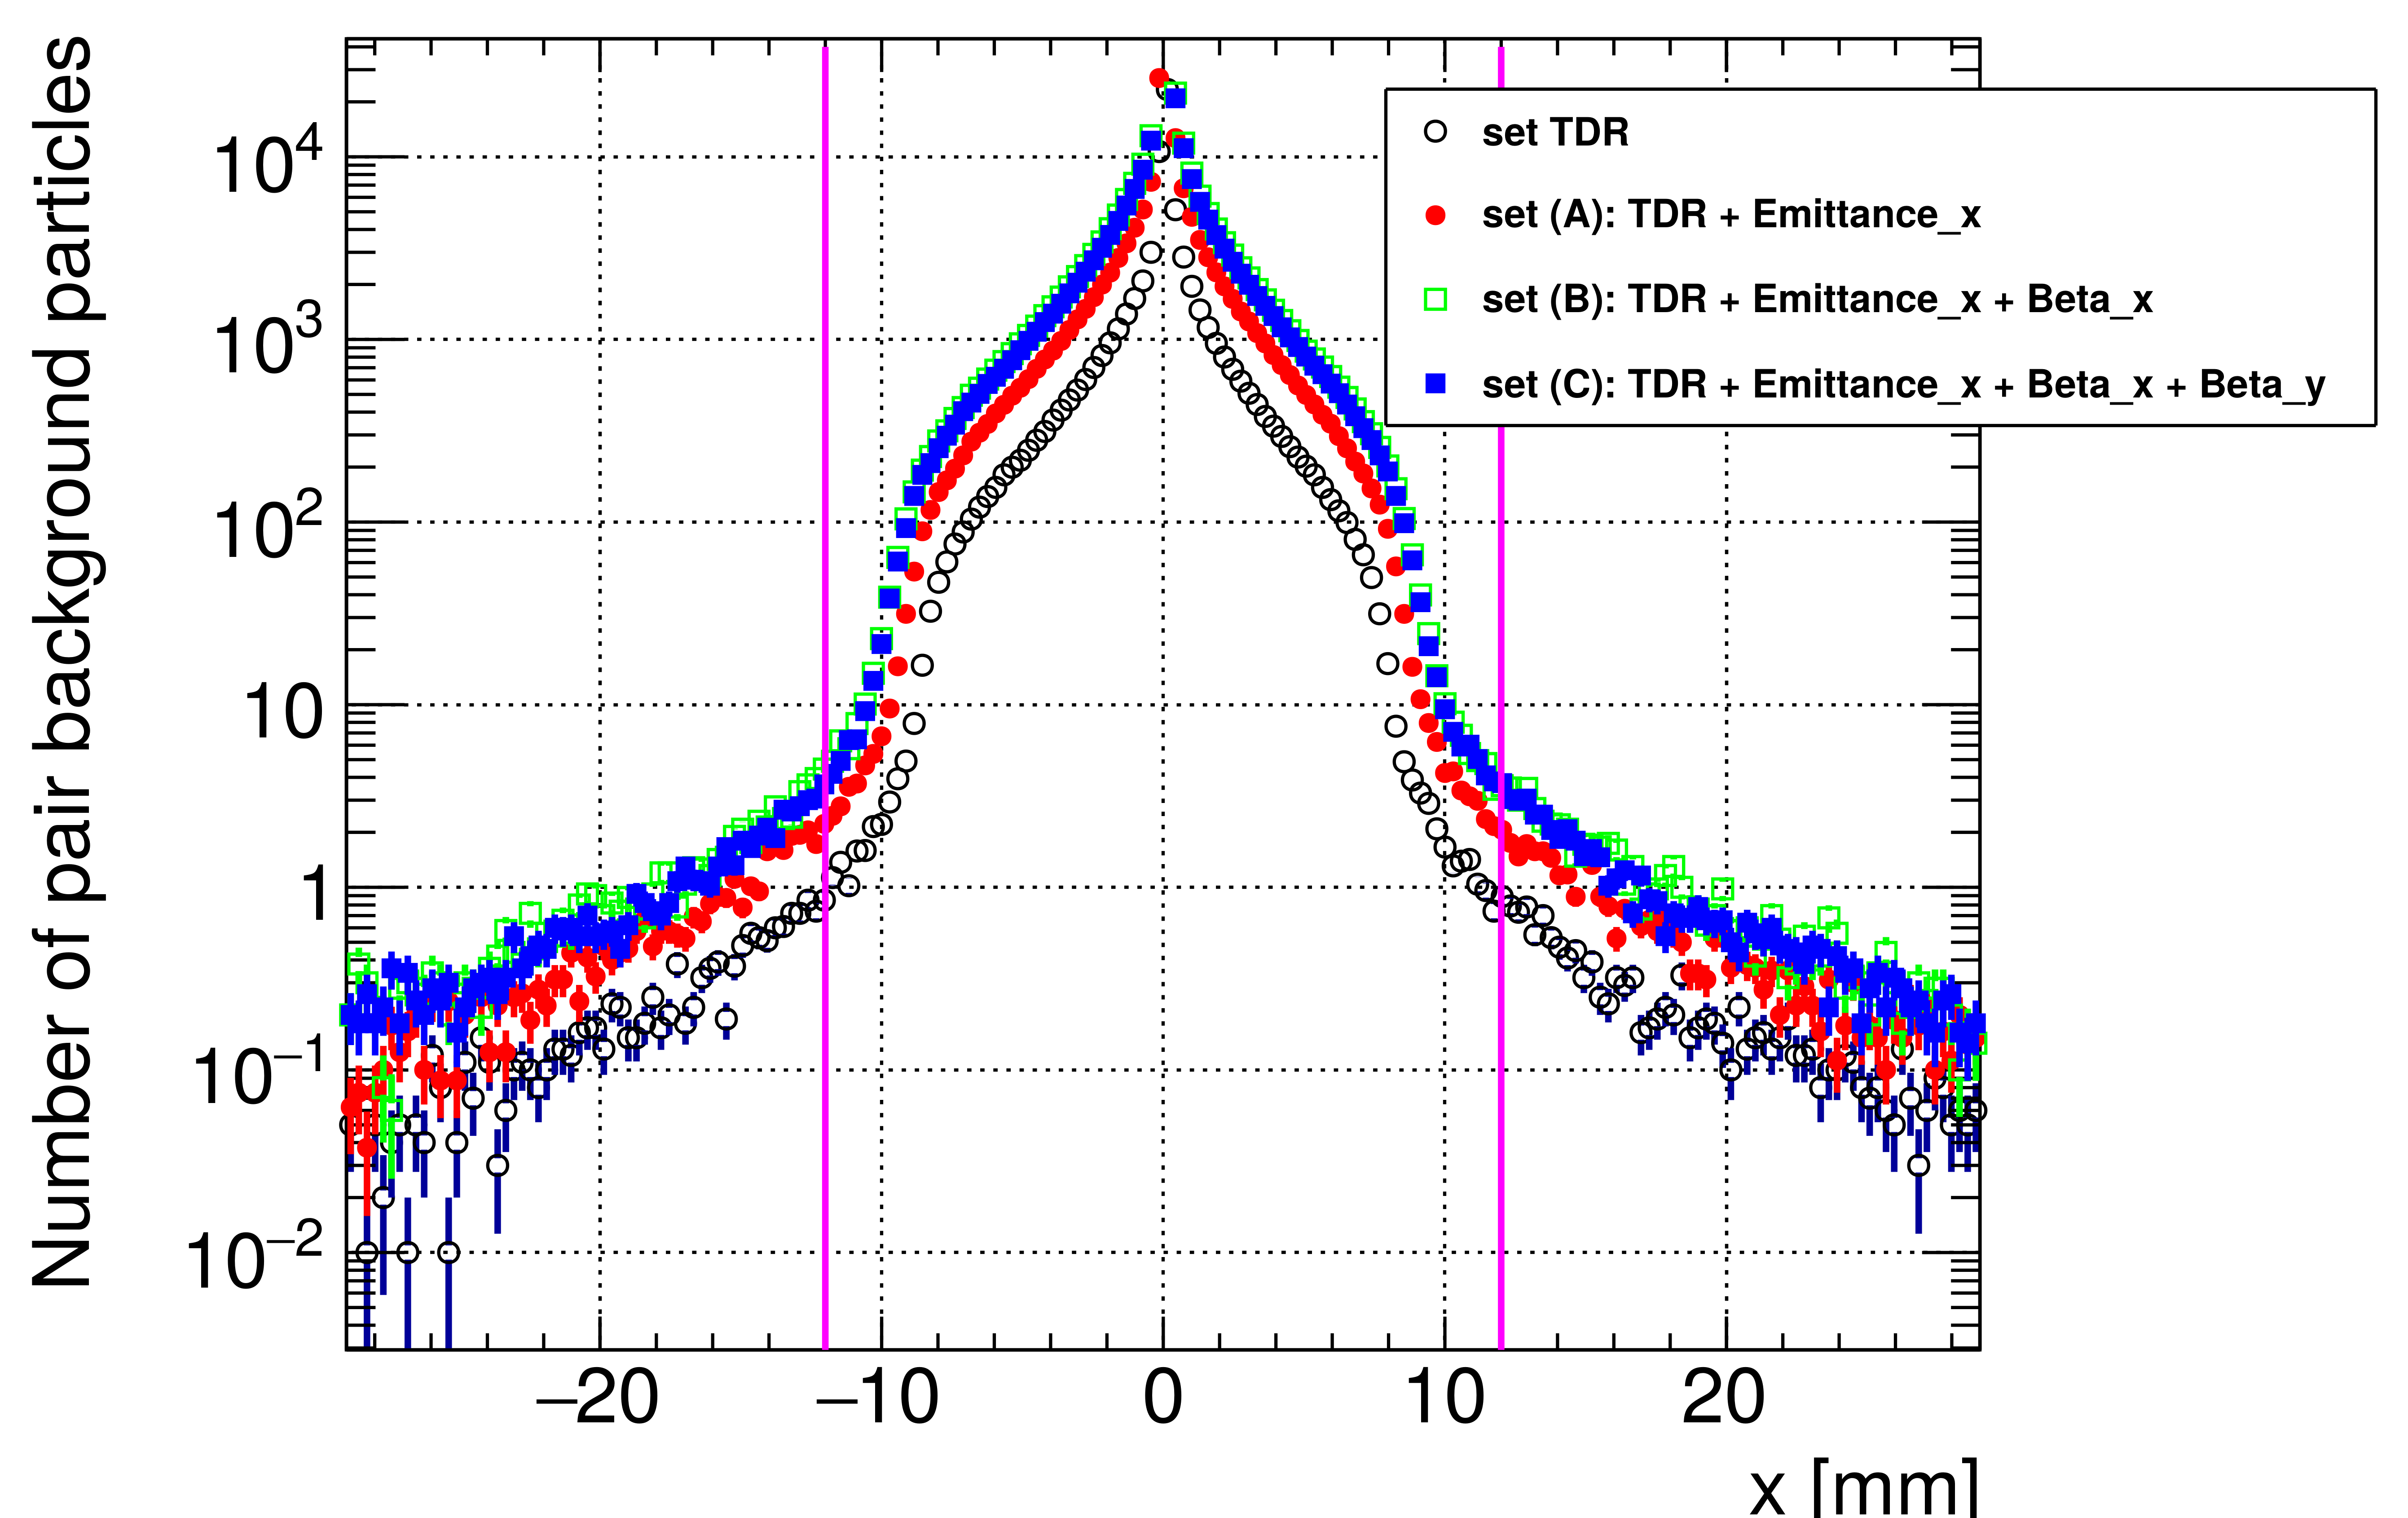
\includegraphics[width=0.7\textwidth]{Figures/Pairs/HelixEnvelope_Projection_Comparison_250GeV_parametersets_LEG.png}
    \caption[Pair background density projection for different ILC250 beam parameter sets]{
    Comparison of the pair background density projection for the four different ILC250 beam parameter sets listed in Table~\ref{tab:ILC250_sets}.
    The plot shows the projected number of pairs along the x-axis for z = \SI[detect-all]{62}{\milli\meter}, which is the z position of the first beam pipe kink.
    The pink vertical lines represent the beam pipe radius at this z position.
    }
    \label{fig:PairBkg:Density_Projection}
\end{figure}

\section{Occupancy studies and buffer depth}
\label{PairBkg:occupancy}
For the vertex detector occupancy studies, the number of hits of every detector cell is counted and translated into an occupancy.
In the following occupancy plots, it can be determined how many detector cells get a certain number of hits.
Knowing that a detector sensor can only store up to a specific number of hits (the so-called buffer depth), the number of dead cells can then be calculated.
A cell is defined to be dead when the buffer of its sensor is already completely filled, and no further hits can be stored.
This is especially important as the detectors for the ILC will read out their buffers only after every bunch train (1312 bunch crossings).
In order to guarantee that cell buffers are not filled only by background hits, a balance has to be found between a sufficient buffer depth and low background levels dependent on the design of the accelerator and the detectors.
In SiD, a rough estimate for an acceptable occupancy for background events is that the sum of all cells with a number of hits greater than or equal to the buffer depth should not exceed \SI{0.01}{\percent} (\num{e-4} of all cells). 
\\Figure~\ref{fig:PairBkg:ILC250_Occupancy} shows the occupancy for all vertex barrel detector layers combined after a full bunch train.
For producing these plots, pair background simulation files for 1312 bunch crossings have been generated with \guineapig, and the number of hits were counted for each cell, summed up over the full bunch train.
A cell size of \SI{20}{\micro\meter}\,x\,\SI{20}{\micro\meter} has been assumed for these calculations.
Plotting the number of cells with a certain amount of hits, and normalizing these numbers by the total number of cells in all vertex detector layers, results in Figure~\ref{fig:PairBkg:ILC250_Occupancy} (a).
It can be directly seen which percentage of all cells get hit a certain number of times.
Comparing the results from the four different ILC250 beam parameter sets, the occupancy of set (A) is raised by a factor of 3 with respect to the baseline set (TDR).
For set (B) and (C), the occupancy is increased by a factor of about 6.
\\Since the readout design for the vertex detector is not yet decided, optimizations based on simulation recommendations can still be made.
In Figure~\ref{fig:PairBkg:ILC250_Occupancy} (b), the number of dead cells are therefore plotted as a function of the assumed buffer depth of the sensors.
The buffer depth states how many hits a sensor can store, before the according cell is blind to any further hits.
The number of these dead cells is calculated from the occupancy plot in Figure ~\ref{fig:PairBkg:ILC250_Occupancy} (a), and depends on the buffer depth.
In the current detector design, the sensors have a buffer depth of four. 
For this value, plot (b) shows that for set (A) \num{8e-6} of all cells in all vertex detector layers are dead, which is an increase with respect to the baseline set of four.
Nevertheless, \num{8e-6} is more than one order of magnitude below the critical limit of \num{e-4} of all cells, which was explained above.
 \begin{figure}[h]
 \centering
  \begin{subfigure}[b]{0.49\textwidth}
   \centering
    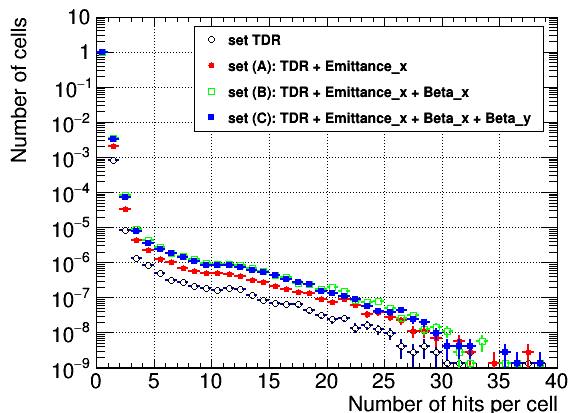
\includegraphics[width=\textwidth]{Figures/Pairs/Occupancy_Comparison_All_layers_wrt_cells_ILC250_Comparison_ALL_SETS_5T_w_antiDiD_LEG.png}
   \caption{Normalized occupancy}
   \end{subfigure}
   \hfill
    \begin{subfigure}[b]{0.49\textwidth}
   \centering
    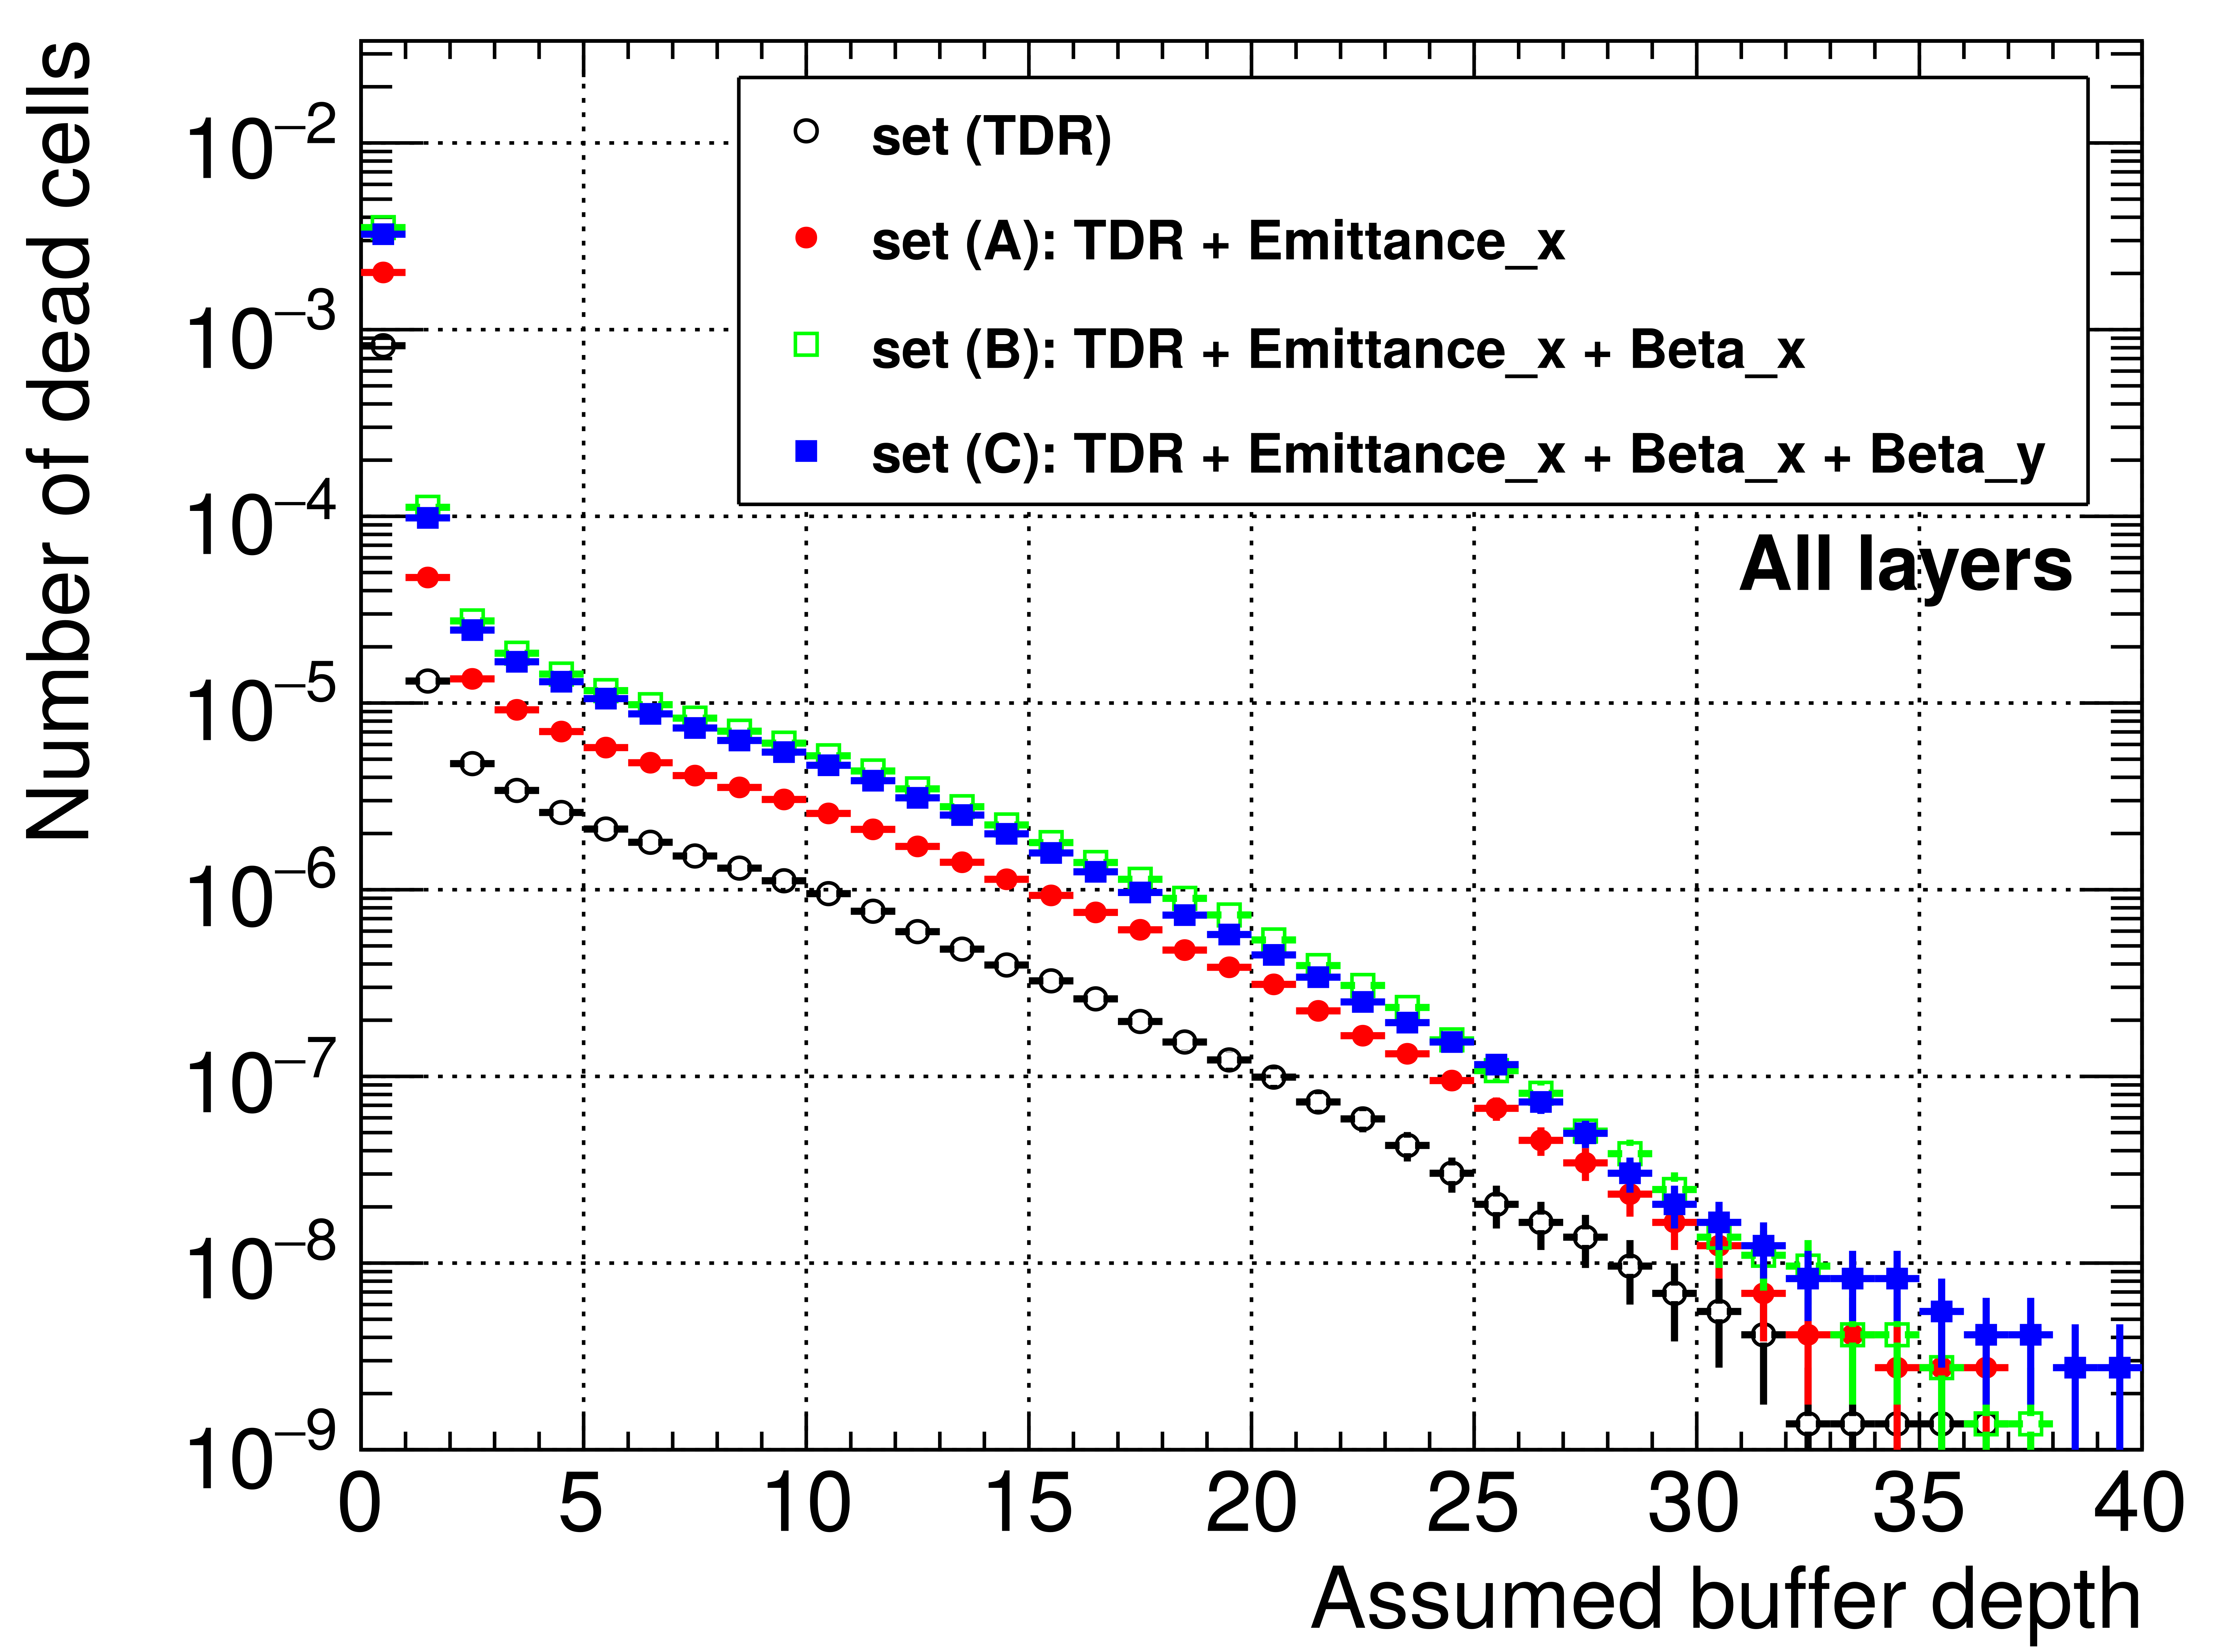
\includegraphics[width=\textwidth]{Figures/Pairs/Occupancy_Comparison_All_layers_deadcells_ILC250_Comparison_ALL_SETS_5T_w_antiDiD_LEG.png}
   \caption{Ratio of dead cells}
   \end{subfigure}
   \caption[Pair background occupancy in the SiD vertex detector for the ILC250]{ILC250 pair background occupancy in the SiD vertex detector for all layers combined, after a full bunch train (1312 bunch crossings).
   Figure (a) shows the occupancy, normalized by the total number of cells of all vertex detector layers.
   Figure (b) shows the ratio of the dead cells with respect to the total number of cells.
   In both figures, the four different beam parameter sets for the ILC250 are compared.
   }
   \label{fig:PairBkg:ILC250_Occupancy}
 \end{figure}
\\Combining the hits of all five vertex barrel detector layers does however not provide a realistic picture of the occupancy in the innermost layer, which is expected to suffer from a larger pair background occupancy than the other layers.
Figure~\ref{fig:PairBkg:ILC250_Occupancy_Layer0} shows then consequently the normalized occupancy and the ratio of dead cells for the innermost vertex detector layer only.
Here in Figure~\ref{fig:PairBkg:ILC250_Occupancy_Layer0} (a), the normalized occupancy in all sets is larger by almost one order of magnitude compared to Figure~\ref{fig:PairBkg:ILC250_Occupancy} (a).
The number of dead cells for a buffer depth of four, shown in Figure~\ref{fig:PairBkg:ILC250_Occupancy_Layer0} (b), is now close to the critical limit of \num{e-4} of all cells.
For set (A), the ratio of dead cells for this buffer depth is about \num{4e-5}.
For sets (B) and (C), the ratio reaches about \num{8e-5} of all cells in this innermost layer.
 \begin{figure}[h]
 \centering
  \begin{subfigure}[b]{0.49\textwidth}
   \centering
    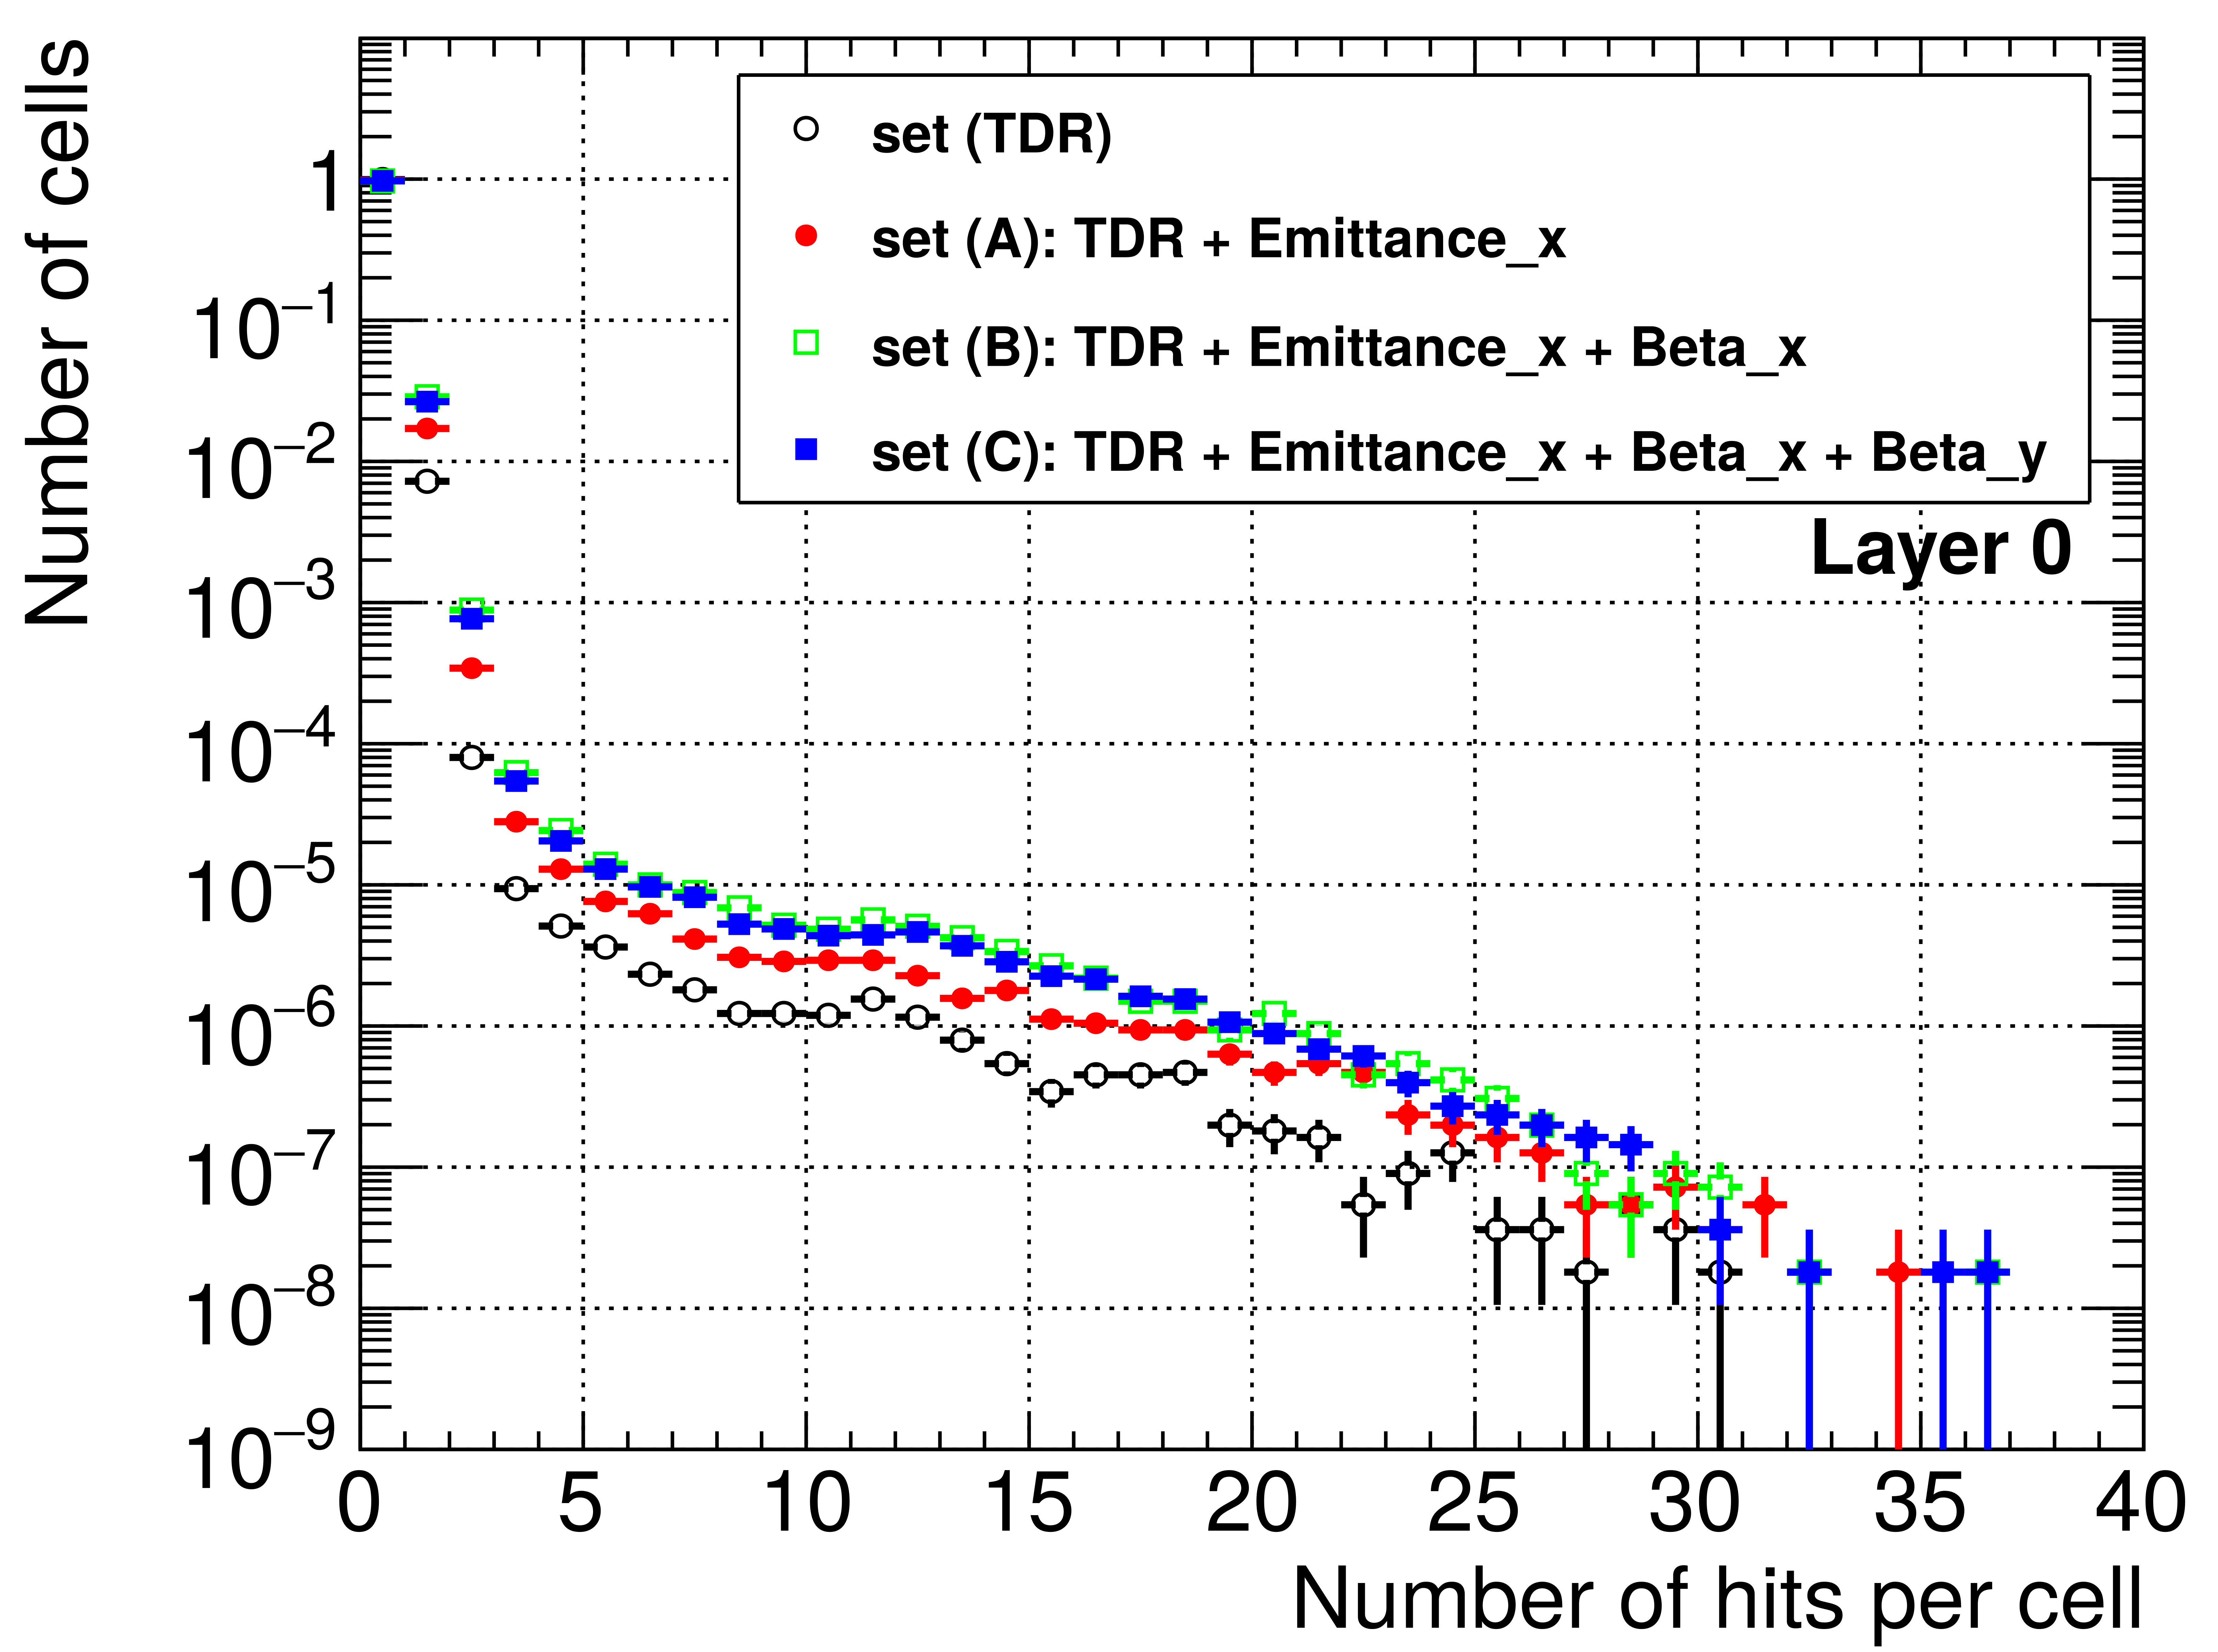
\includegraphics[width=\textwidth]{Figures/Pairs/Occupancy_Comparison_Layer_0_numcells_ILC250_Comparison_ALL_SETS_5T_w_antiDiD_LEG.png}
   \caption{Normalized occupancy}
   \end{subfigure}
   \hfill
    \begin{subfigure}[b]{0.49\textwidth}
   \centering
    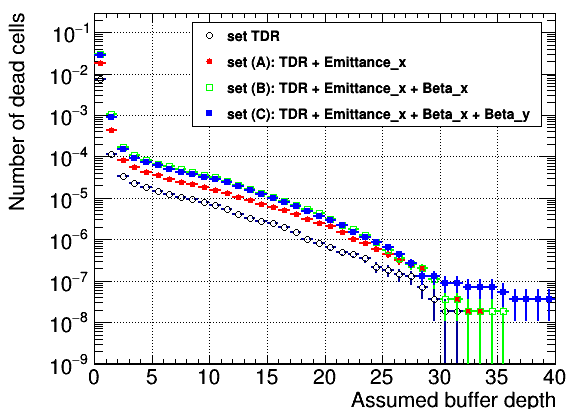
\includegraphics[width=\textwidth]{Figures/Pairs/Occupancy_Comparison_Layer_0_deadcells_ILC250_Comparison_ALL_SETS_5T_w_antiDiD_LEG.png}
   \caption{Ratio of dead cells}
   \end{subfigure}
   \caption[Pair background occupancy in the SiD vertex detector layer 0 for the ILC250]{ILC250 pair background occupancy in the innermost SiD vertex detector layer, after a full bunch train (1312 bunch crossings).
   Figure (a) shows the occupancy, normalized by the total number of cells of the innermost vertex detector layer.
   Figure (b) shows the ratio of the dead cells with respect to the total number of cells.
   In both figures, the four different beam parameter sets for the ILC250 are compared.
   }
   \label{fig:PairBkg:ILC250_Occupancy_Layer0}
 \end{figure}

\begin{itemize}
 \item Occupancy studies for ILC250 parameter sets compared with ILC500 TDR
 \item Occupancy studies for ILC250 parameter sets for different SiD designs (old L*, w/o antiDiD etc) - insert plots
\end{itemize}

\subsection{Hit maps of the SiD subdetectors}
\label{PairBkg:hitmaps}
\todo{Show with projection of hitmaps that there are more hits on edges of VertexBarrel detector (because of helix envelopes)}
%TODO TH1D* histo=Layer_1->ProjectionX("ProjectionX",1,Layer_1->GetNbinsY(),"e")


\section{Hit time distributions}
\label{PairBkg:hittime}

\begin{itemize}
 \item Time distribitution of pairs - redo for ILC250
 \item Plots of particle origins - redo for ILC250
 \item Possible reduction of background through time gates
\end{itemize}

